
\section{Additional Simulation Parameters}
\label{section:add}

\subsection{Constraints and Restraints}
\label{section:config_add}

\subsubsection{Harmonic constraint parameters}

The following describes the parameters for the 
harmonic constraints feature of \NAMD.  Actually, this feature 
should be referred to as harmonic restraints rather than 
constraints, but for historical reasons the terminology of 
harmonic constraints has been carried over from X-PLOR.  
This feature allows a harmonic restraining force to be applied 
to any set of atoms in the simulation.

\begin{itemize}

\item
\NAMDCONFWDEF{constraints}{are constraints active?}{{\tt on} or {\tt off}}{{\tt off}}
{Specifies whether or not harmonic constraints are active.  If it 
is set to {\tt off}, then no harmonic constraints are computed.  
If it is set to {\tt on}, then 
harmonic constraints are calculated using the values specified 
by the parameters {\tt consref}, {\tt conskfile}, {\tt conskcol}, 
and {\tt consexp}.}

\item
\NAMDCONFWDEF{consexp}{exponent for harmonic constraint energy function}{positive, even integer}{2}
{Exponent to be use in the harmonic constraint energy function.  
This value must be a positive integer, and only even values really make 
sense.  This parameter is used only if {\tt constraints} is set to 
{\tt on}.}

\item
\NAMDCONF{consref}{PDB file containing constraint reference positions}{UNIX file name}
{PDB file to use for reference positions for harmonic constraints.  
Each atom that has an active constraint will be constrained about 
the position specified in this file.}

\item
\NAMDCONF{conskfile}{PDB file containing force constant values}{UNIX filename}
{PDB file to use for force constants for 
harmonic constraints.}

\item
\NAMDCONF{conskcol}{column of PDB file containing force constant}{{\tt X}, {\tt Y}, {\tt Z}, {\tt O}, or {\tt B}}
{Column of the PDB file to use for the harmonic constraint force constant.
This parameter may specify any of the floating point fields of the PDB file, 
either X, Y, Z, occupancy, or beta-coupling (temperature-coupling).  
Regardless of which column is used, a value of 0 indicates that the atom 
should not be constrained.  
Otherwise, the value specified is used as the force constant for 
that atom's restraining potential.}

\item
\NAMDCONFWDEF{selectConstraints}{Restrain only selected Cartesian components of the coordinates?}{{\tt on} or {\tt off}}{{\tt off}}
{This option is useful to restrain the positions of atoms to a plane or a line in space. If active,
 this option will ensure that only selected Cartesian components of the coordinates are restrained.
 E.g.: Restraining the positions of atoms to their current z values with no restraints
 in x and y will allow the atoms to move in the x-y plane while retaining their original z-coordinate.
 Restraining the x and y values will lead to free motion only along the z coordinate.}

\item
\NAMDCONFWDEF{selectConstrX}{Restrain X components of coordinates}{{\tt on} or {\tt off}}{{\tt off}}
{Restrain the Cartesian x components of the positions.}
\item
\NAMDCONFWDEF{selectConstrY}{Restrain Y components of coordinates}{{\tt on} or {\tt off}}{{\tt off}}
{Restrain the Cartesian y components of the positions.}
\item
\NAMDCONFWDEF{selectConstrZ}{Restrain Z components of coordinates}{{\tt on} or {\tt off}}{{\tt off}}
{Restrain the Cartesian z components of the positions.}

\end{itemize}

\subsubsection{Fixed atoms parameters}

Atoms may be held fixed during a simulation.  \NAMD\ avoids calculating most interactions in which all affected atoms are fixed unless {\tt fixedAtomsForces} is specified.

\begin{itemize}

\item
\NAMDCONFWDEF{fixedAtoms}{are there fixed atoms?}{{\tt on} or {\tt off}}{{\tt off}}
{Specifies whether or not fixed atoms are present.} 

\item
\NAMDCONFWDEF{fixedAtomsForces}{are forces between fixed atoms calculated?}{{\tt on} or {\tt off}}{{\tt off}}
{Specifies whether or not forces between fixed atoms are calculated.  This option is required to turn fixed atoms off in the middle of a simulation.
These forces will affect the pressure calculation, and you should leave this option off when using constant pressure if the coordinates of the fixed atoms have not been minimized.
The use of constant pressure with significant numbers of fixed atoms is not recommended.}

\item
\NAMDCONFWDEF{fixedAtomsFile}{PDB file containing fixed atom parameters}
{UNIX filename}{{\tt coordinates}}
{PDB file to use for the fixed atom flags for each atom.  
If this parameter is not specified, then 
the PDB file specified by {\tt coordinates} is used.}

\item
\NAMDCONFWDEF{fixedAtomsCol}{column of PDB containing fixed atom parameters}
{{\tt X}, {\tt Y}, {\tt Z}, {\tt O}, or {\tt B}}{{\tt O}} 
{Column of the PDB file to use for the containing fixed atom parameters for 
each atom.  The coefficients can be read from any 
floating point column of the PDB file.  
A value of 0 indicates that the atom is not fixed.}

\end{itemize}

\subsection{Energy Minimization}

\subsubsection{Conjugate gradient parameters}

The default minimizer uses a sophisticated conjugate gradient and
line search algorithm with much better performance than the older
velocity quenching method.
The method of conjugate gradients is used to select successive search
directions (starting with the initial gradient) which eliminate
repeated minimization along the same directions.
Along each direction, a minimum is first bracketed (rigorously bounded)
and then converged upon by either a golden section search, or, when
possible, a quadratically convergent method using gradient information.

For most systems, it just works.

\begin{itemize}

\item
\NAMDCONFWDEF{minimization}{Perform conjugate gradient energy minimization?}{{\tt on} or {\tt off}}{{\tt off}}
{Turns efficient energy minimization {\tt on} or {\tt off}.}

\item
\NAMDCONFWDEF{minTinyStep}{first initial step for line minimizer}{positive decimal}{1.0e-6}
{If your minimization is immediately unstable, make this smaller.}

\item
\NAMDCONFWDEF{minBabyStep}{max initial step for line minimizer}{positive decimal}{1.0e-2}
{If your minimization becomes unstable later, make this smaller.}

\item
\NAMDCONFWDEF{minLineGoal}{gradient reduction factor for line minimizer}{positive decimal}{1.0e-4}
{Varying this might improve conjugate gradient performance.}

\end{itemize}

\subsubsection{Velocity quenching parameters}

You can perform energy minimization using a simple quenching
scheme.   While this algorithm is not the most rapidly convergent, it
is sufficient for most applications.  There are only two parameters
for minimization:  one to activate minimization and another
to specify the maximum movement of any atom.  

\begin{itemize}

\item
\NAMDCONFWDEF{velocityQuenching}{Perform old-style energy minimization?}{{\tt on} or {\tt off}}{{\tt off}}
{Turns slow energy minimization {\tt on} or {\tt off}.}

\item
\NAMDCONFWDEF{maximumMove}{maximum distance an atom can move during each step (\AA)}
{positive decimal}
{$0.75\times\mbox{{\tt cutoff}}/\mbox{{\tt stepsPerCycle}}$}
{Maximum distance that an atom can move during any single timestep of
minimization.  This is to insure that atoms do not go flying off into
space during the first few timesteps when the largest energy conflicts
are resolved.}

\end{itemize}

\subsection{Temperature Control and Equilibration}

\subsubsection{Langevin dynamics parameters}

\NAMD\ is capable
of performing Langevin dynamics, where additional damping and
random forces are introduced to the system.  This capability
is based on that implemented in X-PLOR which is detailed
in the X-PLOR {\it User's Manual} \mycite{(Br\"unger, 1992)}{BRUN92b},
although a different integrator is used.

\begin{itemize}

\item
\NAMDCONFWDEF{langevin}{use Langevin dynamics?}{{\tt on} or {\tt off}}{{\tt off}}
{Specifies whether or not Langevin dynamics active.  
If set to {\tt on}, then the parameter {\tt langevinTemp} must be set 
and the parameters {\tt langevinFile} and {\tt langevinCol} can
optionally be set to control the behavior of this feature.} 

\item
\NAMDCONF{langevinTemp}{temperature for Langevin calculations (K)}{positive decimal}
{Temperature to which atoms affected by Langevin dynamics will be adjusted.  
This temperature will be roughly maintained across the affected atoms 
through the addition of friction and random forces.}

\item
\NAMDCONFWDEF{langevinDamping}{damping coefficient for Langevin dynamics (1/ps)}{positive decimal}{per-atom values from PDB file}
{Langevin coupling coefficient to be applied to all atoms (unless {\tt langevinHydrogen} is {\tt off}, in which case only non-hydrogen atoms are affected).
If not given, a PDB file is used to obtain coefficients for each atom (see {\tt langevinFile} and {\tt langevinCol} below).}

\item
\NAMDCONFWDEF{langevinHydrogen}{Apply Langevin dynamics to hydrogen atoms?}{{\tt on} or {\tt off}}{{\tt on}}
{If {\tt langevinDamping} is set then setting {\tt langevinHydrogen} to {\tt off} will turn off Langevin dynamics for hydrogen atoms.  This parameter has no effect if Langevin coupling coefficients are read from a PDB file.}

\item
\NAMDCONFWDEF{langevinFile}{PDB file containing Langevin parameters}
{UNIX filename}{{\tt coordinates}}
{PDB file to use for the Langevin coupling coefficients for each atom.  
If this parameter is not specified, then 
the PDB file specified by {\tt coordinates} is used.}

\item
\NAMDCONFWDEF{langevinCol}{column of PDB from which to read coefficients}
{{\tt X}, {\tt Y}, {\tt Z}, {\tt O}, or {\tt B}}{{\tt O}} 
{Column of the PDB file to use for the Langevin coupling coefficients for 
each atom.  The coefficients can be read from any 
floating point column of the PDB file.  
A value of 0 indicates that the atom will remain unaffected.}

\end{itemize}

\subsubsection{Temperature coupling parameters}

\NAMD\ is capable
of performing temperature coupling, in which forces are added or 
reduced to simulate the coupling of the system to a heat bath 
of a specified temperature.  
This capability is based on that implemented in X-PLOR which is detailed
in the X-PLOR {\it User's Manual} \mycite{(Br\"unger, 1992)}{BRUN92b}.

\begin{itemize}

\item
\NAMDCONFWDEF{tCouple}{perform temperature coupling?}{{\tt on} or {\tt off}}{{\tt off}}
{Specifies whether or not temperature coupling is active.  
If set to {\tt on}, then the parameter {\tt tCoupleTemp} must be set and 
the parameters {\tt tCoupleFile} and {\tt tCoupleCol} can 
optionally be set to control the behavior of this feature.} 

\item
\NAMDCONF{tCoupleTemp}{temperature for heat bath (K)}{positive decimal}
{Temperature to which atoms affected 
by temperature coupling will be adjusted.  
This temperature will be roughly maintained across the affected atoms 
through the addition of forces.}

\item
\NAMDCONFWDEF{tCoupleFile}{PDB file with tCouple parameters}
{UNIX filename}{{\tt coordinates}}
{PDB file to use for the temperature coupling coefficient for each atom.  
If this parameter is not specified, then 
the PDB file specified by {\tt coordinates} is used.} 

\item
\NAMDCONFWDEF{tCoupleCol}{column of PDB from which to read coefficients}
{{\tt X}, {\tt Y}, {\tt Z}, {\tt O}, or {\tt B}}{{\tt O}} 
{Column of the PDB file to use for the temperature coupling coefficient for 
each atom.  This value can be read from any 
floating point column of the PDB file.  
A value of $0$ indicates that the atom will remain unaffected.}

\end{itemize}

\subsubsection{Temperature rescaling parameters}

\NAMD\ allows equilibration of a system by means of temperature 
rescaling.  Using this method, all of the velocities in the system 
are periodically rescaled so that the entire system is set to the 
desired temperature.  The following parameters specify how often 
and to what temperature this rescaling is performed.  

\begin{itemize}

\item
\NAMDCONF{rescaleFreq}{number of timesteps between temperature rescaling}{positive integer}
{The equilibration feature of \NAMD\ is activated by 
specifying the number of timesteps between each temperature rescaling.  
If this value is given, then the {\tt rescaleTemp} parameter must also 
be given to specify the target temperature. }

\item
\NAMDCONF{rescaleTemp}{temperature for equilibration (K)}{positive decimal}
{The temperature to which all velocities will be rescaled
every {\tt rescaleFreq} timesteps.  
This parameter is valid only if {\tt rescaleFreq} has been set.}

\end{itemize}

\subsubsection{Temperature reassignment parameters}

\NAMD\ allows equilibration of a system by means of temperature 
reassignment.  Using this method, all of the velocities in the system 
are periodically reassigned so that the entire system is set to the 
desired temperature.  The following parameters specify how often 
and to what temperature this reassignment is performed.  

\begin{itemize}

\item
\NAMDCONF{reassignFreq}{number of timesteps between temperature reassignment}{positive integer}
{The equilibration feature of \NAMD\ is activated by 
specifying the number of timesteps between each temperature reassignment.
If this value is given, then the {\tt reassignTemp} parameter must also 
be given to specify the target temperature. }

\item
\NAMDCONFWDEF{reassignTemp}{temperature for equilibration (K)}{positive decimal}{{\tt temperature} if set, otherwise none}
{The temperature to which all velocities will be reassigned
every {\tt reassignFreq} timesteps.  
This parameter is valid only if {\tt reassignFreq} has been set.}

\item
\NAMDCONFWDEF{reassignIncr}{temperature increment for equilibration (K)}{decimal}{0}
{In order to allow simulated annealing or other slow heating/cooling protocols, {\tt reassignIncr} will be added to {\tt reassignTemp} after each reassignment.
(Reassignment is carried out at the first timestep.)  The {\tt reassignHold} parameter may be set to limit the final temperature.
This parameter is valid only if {\tt reassignFreq} has been set.}

\item
\NAMDCONF{reassignHold}{holding temperature for equilibration (K)}{positive decimal}
{The final temperature for reassignment when {\tt reassignIncr} is set; {\tt reassignTemp} will be held at this value once it has been reached.
This parameter is valid only if {\tt reassignIncr} has been set.}

\end{itemize}

\subsection{Boundary Conditions}

In addition to periodic boundary conditions, NAMD provides spherical and
cylindrical boundary potentials to contain atoms in a given volume.
To apply more general boundary potentials written in Tcl, use
{\tt tclBC} as described in Sec.~\ref{section:tclBC}.

\subsubsection{Spherical harmonic boundary conditions}

\NAMD\ provides spherical harmonic boundary conditions.  These 
boundary conditions can consist of a single potential or a 
combination of two potentials.
The following parameters are used to define these boundary conditions.  

\begin{itemize}

\item
\NAMDCONFWDEF{sphericalBC}{use spherical boundary conditions?}{{\tt on} or {\tt off}}{{\tt off}}
{Specifies whether or not spherical boundary conditions 
are to be applied to the system.  If 
set to {\tt on}, then {\tt sphericalBCCenter}, {\tt sphericalBCr1} and {\tt sphericalBCk1} 
must be defined, and {\tt sphericalBCexp1}, {\tt sphericalBCr2}, 
{\tt sphericalBCk2}, and {\tt sphericalBCexp2} can optionally be 
defined.}

\item
\NAMDCONF{sphericalBCCenter}{center of sphere (\AA)}{position}
{Location around which sphere is centered.}

\item
\NAMDCONF{sphericalBCr1}{radius for first boundary condition (\AA)}{positive decimal}
{Distance at which the first potential of the boundary conditions takes
effect.  This distance is a radius from the center.}

\item
\NAMDCONF{sphericalBCk1}{force constant for first potential}{non-zero decimal}
{Force constant for the first harmonic potential.  A positive
value will push atoms toward the center, and a negative
value will pull atoms away from the center.}

\item
\NAMDCONFWDEF{sphericalBCexp1}{exponent for first potential}{positive, even integer}{2}
{Exponent for first boundary potential.  The only likely values to
use are 2 and 4.}

\item
\NAMDCONF{sphericalBCr2}{radius for second boundary condition (\AA)}{positive decimal}
{Distance at which the second potential of the boundary conditions takes
effect.  This distance is a radius from the center.
If this parameter is defined, then {\tt spericalBCk2} must also
be defined.}

\item
\NAMDCONF{sphericalBCk2}{force constant for second potential}{non-zero decimal}
{Force constant for the second harmonic potential.  A positive
value will push atoms toward the center, and a negative
value will pull atoms away from the center.}

\item
\NAMDCONFWDEF{sphericalBCexp2}{exponent for second potential}{positive, even integer}{2}
{Exponent for second boundary potential.  The only likely values to
use are 2 and 4.}

\end{itemize}

\subsubsection{Cylindrical harmonic boundary conditions}

\NAMD\ provides cylindrical harmonic boundary conditions.  These 
boundary conditions can consist of a single potential or a 
combination of two potentials.
The following parameters are used to define these boundary conditions.  

\begin{itemize}

\item
\NAMDCONFWDEF{cylindricalBC}{use cylindrical boundary conditions?}{{\tt on} or {\tt off}}{{\tt off}}
{Specifies whether or not cylindrical boundary conditions 
are to be applied to the system.  If 
set to {\tt on}, then {\tt cylindricalBCCenter}, {\tt cylindricalBCr1}, {\tt cylindricalBCl1} and {\tt cylindricalBCk1} 
must be defined, and {\tt cylindricalBCAxis}, {\tt cylindricalBCexp1}, {\tt cylindricalBCr2}, {\tt cylindricalBCl2},
{\tt cylindricalBCk2}, and {\tt cylindricalBCexp2} can optionally be 
defined.}

\item
\NAMDCONF{cylindricalBCCenter}{center of  cylinder (\AA)}{position}
{Location around which cylinder is centered.}

\item
\NAMDCONF{cylindricalBCAxis}{axis of  cylinder (\AA)}{{\tt x}, {\tt y}, or {\tt z}}
{Axis along which cylinder is aligned.}

\item
\NAMDCONF{cylindricalBCr1}{radius for first boundary condition (\AA)}{positive decimal}
{Distance at which the first potential of the boundary conditions takes
effect along the non-axis plane of the cylinder.}

\item
\NAMDCONF{cylindricalBCl1}{distance along cylinder axis for first boundary condition (\AA)}{positive decimal}
{Distance at which the first potential of the boundary conditions takes
effect along the cylinder axis.}

\item
\NAMDCONF{cylindricalBCk1}{force constant for first potential}{non-zero decimal}
{Force constant for the first harmonic potential.  A positive
value will push atoms toward the center, and a negative
value will pull atoms away from the center.}

\item
\NAMDCONFWDEF{cylindricalBCexp1}{exponent for first potential}{positive, even integer}{2}
{Exponent for first boundary potential.  The only likely values to
use are 2 and 4.}

\item
\NAMDCONF{cylindricalBCr2}{radius for second boundary condition (\AA)}{positive decimal}
{Distance at which the second potential of the boundary conditions takes
effect along the non-axis plane of the cylinder.
If this parameter is defined, then {\tt cylindricalBCl2} and {\tt spericalBCk2} must also
be defined.}

\item
\NAMDCONF{cylindricalBCl2}{radius for second boundary condition (\AA)}{positive decimal}
{Distance at which the second potential of the boundary conditions takes
effect along the cylinder axis.
If this parameter is defined, then {\tt cylindricalBCr2} and {\tt spericalBCk2} must also
be defined.}

\item
\NAMDCONF{cylindricalBCk2}{force constant for second potential}{non-zero decimal}
{Force constant for the second harmonic potential.  A positive
value will push atoms toward the center, and a negative
value will pull atoms away from the center.}

\item
\NAMDCONFWDEF{cylindricalBCexp2}{exponent for second potential}{positive, even integer}{2}
{Exponent for second boundary potential.  The only likely values to
use are 2 and 4.}

\end{itemize}


\subsubsection{Periodic boundary conditions}

\NAMD\ provides periodic boundary conditions in 1, 2 or 3 dimensions.
The following parameters are used to define these boundary conditions.  

\begin{itemize}

\item
\NAMDCONFWDEF{cellBasisVector1}{basis vector for periodic boundaries (\AA)}{vector}{0 0 0}
{Specifies a basis vector for periodic boundary conditions.}

\item
\NAMDCONFWDEF{cellBasisVector2}{basis vector for periodic boundaries (\AA)}{vector}{0 0 0}
{Specifies a basis vector for periodic boundary conditions.}

\item
\NAMDCONFWDEF{cellBasisVector3}{basis vector for periodic boundaries (\AA)}{vector}{0 0 0}
{Specifies a basis vector for periodic boundary conditions.}

\item
\NAMDCONFWDEF{cellOrigin}{center of periodic cell (\AA)}{position}{0 0 0}
{When position rescaling is used to control pressure, this location will remain constant.  Also used as the center of the cell for wrapped output coordinates.}

\item
\NAMDCONF{extendedSystem}{XSC file to read cell parameters from}{file name}
{In addition to .coor and .vel output files, \NAMD\ generates a .xsc (eXtended System Configuration) file which contains the periodic cell parameters and extended system variables, such as the strain rate in constant pressure simulations.  Periodic cell parameters will be read from this file if this option is present, ignoring the above parameters.}

\item
\NAMDCONF{XSTfile}{XST file to write cell trajectory to}{file name}
{\NAMD\ can also generate a .xst (eXtended System Trajectory) file which contains a record of the periodic cell parameters and extended system variables during the simulation.  If {\tt XSTfile} is defined, then {\tt XSTfreq} must also be defined.}

\item
\NAMDCONF{XSTfreq}{how often to append state to XST file}{positive integer}
{Like the {\tt DCDfreq} option, controls how often the extended system configuration will be appended to the XST file.}

\item
\NAMDCONFWDEF{wrapWater}{wrap water coordinates around periodic boundaries?}{on or off}{off}
{Coordinates are normally output relative to the way they were read in.  Hence, if part of a molecule crosses a periodic boundary it is not translated to the other side of the cell on output.  This option alters this behavior for water molecules only.}

\item
\NAMDCONFWDEF{wrapAll}{wrap all coordinates around periodic boundaries?}{on or off}{off}
{Coordinates are normally output relative to the way they were read in.  Hence, if part of a molecule crosses a periodic boundary it is not translated to the other side of the cell on output.  This option alters this behavior for all contiguous clusters of bonded atoms.}

\item
\NAMDCONFWDEF{wrapNearest}{use nearest image to cell origin when wrapping coordinates?}{on or off}{off}
{Coordinates are normally wrapped to the diagonal unit cell centered on the origin.  This option, combined with {\tt wrapWater} or {\tt wrapAll}, wraps coordinates to the nearest image to the origin, providing hexagonal or other cell shapes.}

\end{itemize}

\subsection{Pressure Control}

Constant pressure simulation (and pressure calculation) require periodic
boundary conditions.  Pressure is controlled by dynamically adjusting
the size of the unit cell and rescaling all atomic coordinates (other than
those of fixed atoms) during the simulation.

Pressure values in NAMD output are in bar.
PRESSURE is the pressure calculated based on individual atoms, while
GPRESSURE incorporates hydrogen atoms into the heavier atoms to which
they are bonded, producing smaller fluctuations.
The TEMPAVG, PRESSAVG, and GPRESSAVG are the average of temperature and
pressure values since the previous ENERGY output; for the first step
in the simulation they will be identical to TEMP, PRESSURE, and GPRESSURE.

The phenomenological pressure of bulk matter reflects averaging in both
space and time of the sum of a large positive term (the kinetic pressure,
$nRT/V$), and a large cancelling negative term (the static pressure).
The instantaneous pressure of a simulation cell as simulated by NAMD
will have mean square fluctuations (according to David Case quoting
Section 114 of {\em Statistical Physics} by Landau and Lifshitz)
of $kT/(V \beta)$, where $\beta$ is the compressibility, which is
RMS of roughly 100 bar for a 10,000 atom biomolecular system.
Much larger fluctuations are regularly observed in practice.

The instantaneous pressure for a biomolecular system is well defined for
``internal'' forces that are based on particular periodic images of the
interacting atoms, conserve momentum, and are translationally invariant.
When dealing with externally applied forces such as harmonic constraints,
fixed atoms, and various steering forces, NAMD bases its pressure calculation
on the relative positions of the affected atoms in the input coordinates
and assumes that the net force will average to zero over time.  For time
periods during with the net force is non-zero, the calculated pressure
fluctuations will include a term proportional to the distance to the
affected from the user-defined cell origin.
A good way to observe these effects and to confirm that pressure for
external forces is handled reasonably is to run a constant volume cutoff
simulation in a cell that is larger than the molecular system by at least
the cutoff distance; the pressure for this isolated system should average
to zero over time.

Because NAMD's impluse-basd multiple timestepping system alters the
balance between bonded and non-bonded forces from every timestep to an
average balance over two steps, the calculated pressure on even and odd
steps will be different.  The PRESSAVG and GPRESSAVG fields provide the
average over the non-printed intermediate steps.  If you print energies on
every timestep you will see the effect clearly in the PRESSURE field.

The following options affect all pressure control methods.

\begin{itemize}

\item
\NAMDCONFWDEF{useGroupPressure}{group or atomic quantities}
{{\tt yes} or {\tt no}}{{\tt no}}
{Pressure can be calculated using either the atomic virial and kinetic
energy (the default) or a hydrogen-group based pseudo-molecular
virial and kinetic energy.  The latter fluctuates less and is
required in conjunction with rigidBonds (SHAKE).}

\item
\NAMDCONFWDEF{useFlexibleCell}{anisotropic cell fluctuations}
{{\tt yes} or {\tt no}}{{\tt no}}
{\NAMD\ allows the three orthogonal dimensions of the periodic cell
to fluctuate independently when this option is enabled.}

\item
\NAMDCONFWDEF{useConstantRatio}{constant shape in first two cell dimensions}
{{\tt yes} or {\tt no}}{{\tt no}}
{When enabled, \NAMD\ keeps the ratio of the unit cell in the x-y plane 
constant while allowing fluctuations along all axes.  The {\tt useFlexibleCell} option is required for this option.}

\item
\NAMDCONFWDEF{useConstantArea}{constant area and normal pressure conditions}
{{\tt yes} or {\tt no}}{{\tt no}}
{When enabled, \NAMD\ keeps the dimension of the unit cell in the x-y plane 
constant while allowing fluctuations along the z axis.
This is not currently implemented in Berendsen's method.}

\end{itemize}

\subsubsection{Berendsen pressure bath coupling}

\NAMD\ provides constant pressure simulation using Berendsen's method.  
The following parameters are used to define the algorithm.  

\begin{itemize}

\item
\NAMDCONFWDEF{BerendsenPressure}{use Berendsen pressure bath coupling?}{{\tt on} or {\tt off}}{{\tt off}}
{Specifies whether or not Berendsen pressure bath coupling is active.  
If set to {\tt on}, then the parameters {\tt BerendsenPressureTarget}, {\tt BerendsenPressureCompressibility} and {\tt BerendsenPressureRelaxationTime} must be set 
and the parameter {\tt BerendsenPressureFreq} can
optionally be set to control the behavior of this feature.} 

\item
\NAMDCONF{BerendsenPressureTarget}{target pressure (bar)}{positive decimal}
{Specifies target pressure for Berendsen's method.
A typical value would be 1.01325 bar, atmospheric pressure at sea level.}

\item
\NAMDCONF{BerendsenPressureCompressibility}{compressibility (bar$^{-1}$)}{positive decimal}
{Specifies compressibility for Berendsen's method.
A typical value would be 4.57E-5 bar$^{-1}$, corresponding to liquid water.
The higher the compressibility, the more volume will be adjusted for a
given pressure difference.
The compressibility and the relaxation time appear only as a ratio in the
dynamics, so a larger compressibility is equivalent to a smaller relaxation
time.}

\item
\NAMDCONF{BerendsenPressureRelaxationTime}{relaxation time (fs)}{positive decimal}
{Specifies relaxation time for Berendsen's method.
If the instantaneous pressure did not fluctuate randomly during a simulation
and the compressibility estimate was exact then
the inital pressure would decay exponentially to the target pressure with
this time constant.
Having a longer relaxation time results in more averaging over pressure
measurements and hence smaller fluctuations in the cell volume.
A reasonable choice for relaxation time would be 100 fs.
The compressibility and the relaxation time appear only as a ratio in the
dynamics, so a larger compressibility is equivalent to a smaller relaxation
time.}

\item
\NAMDCONFWDEF{BerendsenPressureFreq}{how often to rescale positions}{positive multiple of {\tt nonbondedFrequency} and {\tt fullElectFrequency}}{{\tt nonbondedFrequency} or {\tt fullElectFrequency} if used}
{Specifies number of timesteps between position rescalings for Berendsen's method.
Primarily to deal with multiple timestepping integrators, but also to reduce
cell volume fluctuations, cell rescalings can occur on a longer interval.
This could reasonably be between 1 and 20 timesteps, but the relaxation time
should be at least ten times larger.
}

\end{itemize}

\subsubsection{Nos\'{e}-Hoover Langevin piston pressure control}

\NAMD\ provides constant pressure simulation using a modified Nos\'{e}-Hoover method in which Langevin dynamics is used to control fluctuations in the barostat.
This method should be combined with a method of temperature control, such as Langevin dynamics, in order to simulate the NPT ensemble.

The Langevin piston Nose-Hoover method in NAMD is a combination of the
Nose-Hoover constant pressure method as described in 
GJ Martyna, DJ Tobias and ML Klein, "Constant pressure molecular dynamics
algorithms", J. Chem. Phys 101(5), 1994,
with piston fluctuation control implemented using Langevin dynamics as in
SE Feller, Y Zhang, RW Pastor and BR Brooks, "Constant pressure molecular
dynamics simulation: The Langevin piston method", J. Chem. Phys. 103(11),
1995.

The equations of motion are:
\begin{eqnarray*}
       r' &=& p/m + e' r  \\
       p' &=& F - e' p - g p + R \\
       V' &=& 3 V e' \\
       e'' &=& 3V/W (P - P_0) - g_e e' + R_e/W  \\
       W &=&  3 N \tau^2 k T  \\
       <R^2> &=& 2 m g k T / h \\
       \tau &=& {\rm oscillation period} \\
       <R_e^2> &=& 2 W g_e k T / h
\end{eqnarray*}
Here, $W$ is the mass of piston, $R$ is noise on atoms, and $R_e$ is
the noise on the piston.

The user specifies the desired pressure, oscillation and decay times
of the piston, and temperature of the piston.  The compressibility of  
the system is not required.  In addition, the user specifies the
damping coefficients and temperature of the atoms for Langevin dynamics.

The following parameters are used to define the algorithm.  

\begin{itemize}

\item
\NAMDCONFWDEF{LangevinPiston}{use Langevin piston pressure control?}{{\tt on} or {\tt off}}{{\tt off}}
{Specifies whether or not Langevin piston pressure control is active.  
If set to {\tt on}, then the parameters {\tt LangevinPistonTarget}, {\tt LangevinPistonPeriod}, {\tt LangevinPistonDecay} and {\tt LangevinPistonTemp} must be set.}

\item
\NAMDCONF{LangevinPistonTarget}{target pressure (bar)}{positive decimal}
{Specifies target pressure for Langevin piston method.
A typical value would be 1.01325 bar, atmospheric pressure at sea level.}

\item
\NAMDCONF{LangevinPistonPeriod}{oscillation period (fs)}{positive decimal}
{Specifies barostat oscillation time scale for Langevin piston method.
If the instantaneous pressure did not fluctuate randomly during a simulation
and the decay time was infinite (no friction) then the cell volume would
oscillate with this angular period.
Having a longer period results in more averaging over pressure measurements
and hence slower fluctuations in the cell volume.
A reasonable choice for the piston period would be 200 fs.
}

\item
\NAMDCONF{LangevinPistonDecay}{damping time scale (fs)}{positive decimal}
{Specifies barostat damping time scale for Langevin piston method.
A value larger than the piston period would result in underdamped
dynamics (decaying ringing in the cell volume) while a smaller value
approaches exponential decay as in Berendsen's method above.
A smaller value also corresponds to larger random forces with increased
coupling to the Langevin temperature bath.
Typically this would be chosen equal to or smaller than the piston period,
such as 100 fs.
}

\item
\NAMDCONF{LangevinPistonTemp}{noise temperature (K)}{positive decimal}
{Specifies barostat noise temperature for Langevin piston method.
This should be set equal to the target temperature for the chosen method of temperature control.}

\item
\NAMDCONFWDEF{SurfaceTensionTarget}{Surface tension target (dyn/cm)}
{decimal}{0.0}{Specifies surface tension target.  Must be used with 
{\tt useFlexibleCell} and periodic boundary conditions.  The pressure 
specified in {\tt LangevinPistonTarget} becomes the pressure along the z
axis, and surface tension is applied in the x-y plane.}

\item
\NAMDCONFWDEF{StrainRate}{initial strain rate}{decimal triple (x y z)}
{0. 0. 0.}
{Optionally specifies the initial strain rate for pressure control.
Is overridden by value read from file specified with {\tt extendedSystem}.
There is typically no reason to set this parameter.}

\item
\NAMDCONFWDEF{ExcludeFromPressure}{Should some atoms be excluded from pressure
rescaling?}{{\tt on} or {\tt off}}{{\tt off}}
{Specifies whether or not to exclude some atoms from pressure rescaling.  The
coordinates and velocites of such atoms are not rescaled during constant
pressure simulations, though they do contribute to the virial calculation. 
May be useful for membrane protein simulation.  EXPERIMENTAL.}

\item
\NAMDCONFWDEF{ExcludeFromPressureFile}{File specifying excluded atoms}
{PDB file}{coordinates file}
{PDB file with one column specifying which atoms to exclude from pressure
rescaling.  Specify 1 for excluded and 0 for not excluded.}

\item
\NAMDCONFWDEF{ExcludeFromPressureCol}{Column in PDB file for specifying
excluded atoms}{O, B, X, Y, or Z}{O}
{Specifies which column of the pdb file to check for excluded atoms.}

\end{itemize}

\subsection{Applied Forces and Analysis}

There are several ways to apply external forces to simulations with \NAMD.
These are described below.


\subsubsection{Constant Forces}

NAMD provides the ability to apply constant forces to some atoms.
There are two parameters that control this feature.

\begin{itemize}

\item
\NAMDCONFWDEF{constantforce}{Apply constant forces?}{yes or no}{no}
{Specifies whether or not constant forces are applied.}

\item
\NAMDCONF{consforcefile}{PDB file containing forces to be applied}{UNIX filename}
{
The X, Y, Z and occupancy (O) fields of this file are read to
determine the constant force vector of each atom, which is
(X,Y,Z)*O, in unit of kcal/(mol*\AA). The occupancy (O) serves as
a scaling factor, which could expand the range of the force
applied. (One may be unable to record very large or very small
numbers in the data fields of a PDB file due to limited space).
Zero forces are ignored.

Specifying {\tt consforcefile} is optional; constant forces may be specifed
or updated between runs by using the consForceConfig command.
}

\end{itemize}


\subsubsection{External Electric Field}

\NAMD\ provides the ability to apply a constant electric field to the molecular
system being simulated.
Energy due to the external field will be reported in the MISC column
and may be discontinuous in simulations using periodic boundary conditions if,
for example, a charged hydrogen group moves outside of the central cell.
There are two parameters that control this feature.

\begin{itemize}

\item
\NAMDCONFWDEF{eFieldOn}{apply electric field?}{{\tt yes} or {\tt no}}{{\tt no}}
{Specifies whether or not an electric field is applied.}

\item
\NAMDCONF{eField}{electric field vector}{vector of decimals (x y z)}
{Vector which describes the electric field to be applied.
Units are ${\rm kcal} / ({\rm mol \; \AA} \; e)$, which is natural for simulations.
This parameter may be changed between {\tt run} commands, allowing a square
wave or other approximate wave form to be applied.}

\end{itemize}


\subsubsection{Moving Constraints}

Moving constraints feature works in conjunction with the Harmonic
Constraints (see an appropriate section of the User's guide).
The reference positions of all constraints
will move according to
\begin{equation}
\label{eq:smdrefpos}
   \vec r(t) \; = \; \vec r_0 \, + \, \vec v t \,.
\end{equation}

A velocity vector $\vec v$ ({\tt movingConsVel}) needs to be specified.

The way the moving constraints work is that the moving reference
position is calculated every integration time step using
Eq.~\ref{eq:smdrefpos}, where $\vec v$ is in \AA/timestep, and $t$ is the
current timestep (i.e., {\tt firstTimestep} plus however many
timesteps have passed since the beginning of \NAMD\ run). Therefore,
one should be careful when restarting simulations to appropriately
update the {\tt firstTimestep} parameter in the \NAMD\ configuration
file or the reference position specified in the reference PDB file.

\noindent {\bf NOTE: } \NAMD\ actually calculates the constraints
potential with $U = k (x-x_0)^d$ and the force with $F = d k (x-x_0)$,
where $d$ is the exponent {\tt consexp}. The result is that if one
specifies some value for the force constant $k$ in the PDB file,
effectively, the force constant is $2 k$ in calculations. This caveat
was removed in SMD feature.

The following parameters describe the parameters for the
moving harmonic constraint feature of \NAMD.

\begin{itemize}

\item
\NAMDCONFWDEF{movingConstraints}{Are moving constraints active}
{{\tt on} or {\tt off}}{{\tt off}}
{Should moving restraints be applied to the system. If set
to {\tt on}, then  {\tt movingConsVel} must be defined.
May not be used with {\tt rotConstraints}.}

\item
\NAMDCONF{movingConsVel}{Velocity of the reference position movement}
{vector in \AA/timestep}
{The velocity of the reference position movement. Gives both absolute
value and direction}

\end{itemize}

\subsubsection{Rotating Constraints}

The constraints parameters are specified in the same manner as for
usual (static) harmonic constraints. The reference positions of all
constrained atoms are then rotated with a given angular velocity
about a given axis. If the force constant of the constraints is
sufficiently
large, the constrained atoms will follow their reference positions.

A rotation matrix $M$ about the axis unit vector $v$ is calculated every
timestep
for the angle of rotation corresponding to the current timestep.
    angle = $\Omega t$,
where $\Omega$ is the angular velocity of rotation.

From now on, all quantities are 3D vectors, except the matrix $M$ and the
force constant $K$.

The current reference position $R$ is calculated from the initial
reference
position $R_0$ (at $t=0$),
    $R = M (R_0 - P) + P$,
where $P$ is the pivot point.

%geometry of rotation:
%
%
%
%                        * R
%                      / |
%                    /   |
%                  /     | normal to axis
%                /       |
%            P /         |
%        ----*--->-------*---------------------> axis
%                v       N

Coordinates of point N can be found as
   $N = P + ( (R - P) \cdot v ) v$.
Normal from the atom pos to the axis is, similarly,
   normal $= ( P + ( (X - P) \cdot v ) v ) - X$
The force is, as usual,
   $F = K (R - X)$;
This is the force applied to the atom in NAMD (see below).
NAMD does not know anything about the torque
applied. However, the torque applied to the atom can be calculated
as a vector product
   torque $= F \times normal$
Finally, the torque applied to the atom with respect to the axis
is the projection of the torque on the axis, i.e.,
   $torque_{proj} = torque \cdot v$

If there are atoms that have to be constrained, but not moved,
this implementation is not suitable, because it will move {\em all}
reference positions.

Only one of the moving and rotating constraints can be used at a
time.

Using very soft springs for rotating constraints leads to the system
   lagging behind the reference positions, and then the force is applied
   along a direction different from the "ideal" direction along the
   circular path.

Pulling on N atoms at the same time with a spring of stiffness K
   amounts to pulling on the whole system by a spring of stiffness NK,
   so the overall behavior of the system is as if you are pulling with a
   very stiff spring if N is large.

In both moving and rotating constraints the force constant that you
   specify in the constraints pdb file is multiplied by 2 for the force
   calculation, i.e., if you specified $K = 0.5 \; {\rm kcal}/{\rm mol}/{\rm \AA}^2$ in the pdb
file,
   the force actually calculated is $F = 2 K (R-X) = 1 \; {\rm kcal}/{\rm mol}/{\rm \AA}^2 \; (R-X)$.
   SMD feature of namd2 does the calculation without multiplication of
the
   force constant specified in the config file by 2.


\begin{itemize}

\item
\NAMDCONFWDEF{rotConstraints}{Are rotating constraints active}
{{\tt on} or {\tt off}}{{\tt off}}
{Should rotating restraints be applied to the system. If set
to {\tt on}, then {\tt rotConsAxis}, {\tt rotConsPivot} and
{\tt rotConsVel} must be defined.
May not be used with {\tt movingConstraints}.}

\item
\NAMDCONF{rotConsAxis}{Axis of rotation}
{vector (may be unnormalized)}
{Axis of rotation. Can be any vector. It gets
normalized before use. If the vector is 0,
no rotation will be performed, but the calculations
will still be done.}

\item
\NAMDCONF{rotConsPivot}{Pivot point of rotation}
{position in \AA}
{Pivot point of rotation. The rotation axis vector
only gives the direction of the axis. Pivot point
places the axis in space, so that the axis goes
through the pivot point.}

\item
\NAMDCONF{rotConsVel}{Angular velocity of rotation}
{rate in degrees per timestep}
{Angular velocity of rotation, degrees/timestep.}

\end{itemize}


\subsubsection{Steered Molecular Dynamics (SMD)}

The SMD feature is independent from the harmonic constraints, although it
follows the same ideas.  In both SMD and harmonic constraints, one specifies
a PDB file which indicates which atoms are 'tagged' as constrained.  The PDB
file also gives initial coordinates for the constraint positions.  One also
specifies such parameters as the force constant(s) for the constraints, 
and the velocity with which the constraints move.  

There are two major differences between SMD and
harmonic constraints:
\begin{itemize}
\item In harmonic constraints, each tagged atom is harmonically constrained
  to a reference point which moves with constant velocity.  In SMD, it is
  the {\em center of mass} of the tagged atoms which is constrained to move
  with constant velocity.

\item In harmonic constraints, each tagged atom is constrained in all three
  spatial dimensions.  In SMD, tagged atoms are constrained {\em only along
  the constraint direction}.
\end{itemize}

The center of mass of the SMD atoms will be harmonically constrained with 
force constant $k$ ({\tt SMDk}) to move with velocity $v$ ({\tt SMDVel}) in 
the direction $\vec n$ ({\tt SMDDir}).  SMD thus results in the following
potential being applied to the system:
\begin{equation}
\label{eq:SMDpotential}
U(\vec r_1, \vec r_2, ..., t) \; = \; \frac{1}{2} 
  k\left[vt - (\vec R(t) - \vec R_0)\cdot \vec n \right]^2.
\end{equation}
Here, $t \equiv N_{ts} dt$ where $N_{ts}$ is the number of elapsed timesteps
in the simulation and $dt$ is the size of the timestep in femtoseconds.
Also, $\vec R(t)$ is the current center of mass of the SMD atoms and $R_0$ is
the initial center of mass as defined by the coordinates in {\tt SMDFile}.
Vector $\vec n$ is normalized by \NAMD\ before being used.  

\paragraph*{Output}

\NAMD\ provides output of the current SMD data. The frequency of
output is specified by the {\tt SMDOutputFreq} parameter in the
configuration file. Every {\tt SMDOutputFreq} timesteps \NAMD\ will
print the current timestep, current position of the center of mass of the
restrained atoms, and
the current force applied to the center of mass (in piconewtons, pN).
The output line starts with word {\tt SMD}

\paragraph*{Parameters}

The following parameters describe the parameters for the 
SMD feature of \NAMD.
\begin{itemize}
\item 
\NAMDCONFWDEF{SMD}{Are SMD features active}
{{\tt on} or {\tt off}}{{\tt off}}
{Should SMD harmonic constraint be applied to the system. If set 
to {\tt on}, then  {\tt SMDk}, {\tt SMDFile}, {\tt SMDVel}, and
{\tt SMDDir} must be defined.  Specifying {\tt SMDOutputFreq} 
is optional.}

\item
\NAMDCONF{SMDFile}{SMD constraint reference position}
{UNIX filename} {File to use for the initial reference position for the SMD
harmonic constraints.  All atoms in this PDB file with a nonzero value in the
{\em occupancy} column will be tagged as SMD atoms.  The coordinates of the
tagged SMD atoms will be used to calculate the initial center of mass.
During the simulation, this center of mass will move with velocity
{\tt SMDVel} in the direction {\tt SMDDir}. The actual atom order in this PDB
file must match that in the structure or coordinate file, since the atom
number field in this PDB file will be ignored.}

\item
\NAMDCONF{SMDk}{force constant to use in SMD simulation}
{positive real}
{SMD harmonic constraint force constant. Must be specified in
kcal/mol/\AA$^2$. The conversion factor is 1 kcal/mol = 69.479 pN \AA.} 

\item
\NAMDCONF{SMDVel}{Velocity of the SMD reference position movement}
{nonzero real, \AA/timestep}
{The velocity of the SMD center of mass movement. Gives the absolute
value.}

\item
\NAMDCONF{SMDDir}{Direction of the SMD center of mass movement}
{non-zero vector}
{The direction of the SMD reference position movement. The vector does
not have to be normalized, it is normalized by \NAMD\ before being used.}

\item
\NAMDCONFWDEF{SMDOutputFreq}{frequency of SMD output}
{positive integer}{1} {The frequency in timesteps with which the
current SMD data values are printed out.}
\end{itemize}


\subsubsection{Interactive Molecular Dynamics (IMD)}

\NAMD\ now works directly with \VMD\ to allow you to view and interactively
steer your simulation.  With IMD enabled, you can connect to NAMD at any
time during the simulation to view the current state of the system or perform
interactive steering. 

\begin{itemize}
\item
\NAMDCONFWDEF{IMDon}{is IMD active?}{{\tt on} or {\tt off}}{{\tt off}}
{Specifies whether or not to listen for an IMD connection.}

\item
\NAMDCONF{IMDport}{port number to expect a connection on}
{positive integer}
{This is a free port number on the machine that node 0 is running on.
This number will have to be entered into \VMD.}

\item
\NAMDCONF{IMDfreq}{timesteps between sending coordinates}
{positive integer}
{This allows coordinates to be sent less often, which may increase
\NAMD\ performance or be necessary due to a slow network.}

\item 
\NAMDCONFWDEF{IMDwait}{wait for an IMD connection?}{{\tt yes} or {\tt no}}{{\tt no}}
{If {\tt no}, NAMD will proceed with calculations whether a connection is
present or not.  If {\tt yes}, NAMD will pause at startup until a connection is
made, and pause when the connection is lost.}

\item 
\NAMDCONFWDEF{IMDignore}{ignore interactive steering forces}{{\tt yes} or {\tt no}}{{\tt no}}
{If {\tt yes}, NAMD will ignore any steering forces generated by \VMD\ to allow
a simulation to be monitored without the possibility of perturbing it.}

\end{itemize}


\subsubsection{Tcl Forces and Analysis}

\NAMD\ provides a limited Tcl scripting interface designed for applying forces and performing on-the-fly analysis.
This interface is efficient if only a few coordinates, either of individual atoms or centers of mass of groups of atoms, are needed.
In addition, information must be requested one timestep in advance.
To apply forces individually to a potentially large number of atoms, use
{\tt tclBC} instead as described in Sec.~\ref{section:tclBC}.
The following configuration parameters are used to enable the Tcl interface:

\begin{itemize}

\item
\NAMDCONFWDEF{tclForces}{is Tcl interface active?}{{\tt on} or {\tt off}}{{\tt off}}
{Specifies whether or not Tcl interface is active.  If it 
is set to {\tt off}, then no Tcl code is executed.  
If it is set to {\tt on}, then Tcl code specified in
{\tt tclForcesScript} parameters is executed.}

\item
\NAMDCONF{tclForcesScript}{input for Tcl interface}{file or \{script\}}
{Must contain either the name of a Tcl script file or the script 
itself between \{ and \} (may include multiple lines).
This parameter may occur multiple times and scripts will be executed
in order of appearance.
The script(s) should perform any required initialization on the Tcl interpreter, including requesting data needed during the first timestep, and define a procedure {\tt calcforces \{ \}} to be called every timestep.
}

\end{itemize}

At this point only low-level commands are defined.
In the future this list will be expanded.  Current commands are:

\begin{itemize}

\item
{\tt print <anything>} \\
This command should be used instead of {\tt puts} to display output.
For example, ``\verb&print Hello World&''.

\item
{\tt atomid <segname> <resid> <atomname>} \\
Determines atomid of an atom from its segment, residue, and name.
For example, ``{\tt atomid br 2 N}''.

\item
{\tt addatom <atomid>} \\
Request coordinates of this atom for next force evaluation, and
the calculated total force on this atom for current force evaluation.
Request remains in effect until {\tt clearconfig} is called.
For example, ``{\tt addatom 4}'' or ``{\tt addatom [atomid br 2 N]}''.

\item
{\tt addgroup <atomid list>} \\
Request center of mass coordinates of this group for next force evaluation.
Returns a group ID which is of the form {\tt gN} where {\tt N} is a small integer.
This group ID may then be used to find coordinates and apply forces just like a regular atom ID.
Aggregate forces may then be applied to the group as whole.
Request remains in effect until {\tt clearconfig} is called.
For example, ``{\tt set groupid [addgroup \{ 14 10 12 \}]}''.

\item
{\tt clearconfig} \\
Clears the current list of requested atoms.  After {\tt clearconfig},
calls to {\tt addatom} and {\tt addgroup} can be used to build a new
configuration.

\item
{\tt loadcoords <varname>} \\
Loads requested atom and group coordinates (in \AA) into a local array.
{\tt loadcoords} should only be called from within the {\tt calcforces} procedure.
For example, ``{\tt loadcoords p}'' and ``{\tt print \$p(4)}''.

\item
{\tt loadforces <varname>} \\
Loads the forces applied in the previous timestep (in kcal mol$^{-1}$
\AA$^{-1}$) into a local array.
{\tt loadforces} should only be called from within the {\tt
calcforces} procedure.
For example, ``{\tt loadforces f}'' and ``{\tt print \$f(4)}''.

\item
{\tt loadtotalforces <varname>} \\
Loads the total forces on each requested atom in the previous
time step (in kcal mol$^{-1}$\AA$^{-1}$) into a local array. The
total force also includes external forces. Note that the
``{\tt loadforces}'' command returns external forces applied by
the user. Therefore, one can subtract the external force on an
atom from the total force on this atom to get the pure force
arising from the simulation system.

\item
{\tt loadmasses <varname>} \\
Loads requested atom and group masses (in amu) into a local array.
{\tt loadmasses} should only be called from within the {\tt calcforces} procedure.
For example, ``{\tt loadcoords m}'' and ``{\tt print \$m(4)}''.

\item
{\tt addforce <atomid|groupid> <force vector>} \\
Applies force (in kcal mol$^{-1}$ \AA$^{-1}$) to atom or group.
{\tt addforce} should only be called from within the {\tt calcforces} procedure.
For example, ``\verb!addforce $groupid { 1. 0. 2. }!''.

\item
{\tt addenergy <energy (kcal/mol)>} \\
This command adds the specified energy to the MISC column (and
hence the total energy) in the energy output. For normal runs,
the command does not affect the simulation trajectory at all, and
only has an artificial effect on its energy output. However, it
can indeed affect minimizations.

\end{itemize}

With the commands above and the functionality of the Tcl language,
one should be able to perform any on-the-fly analysis and
manipulation. To make it easier to perform certain tasks,
some Tcl routines are provided below.

Several vector routines ({\tt vecadd}, {\tt vecsub}, {\tt vecscale})
from the VMD Tcl interface are defined. Please refer to VMD
manual for their usage.

The following routines take atom coordinates as input, and return
some geometry parameters (bond, angle, dihedral).

\begin{itemize}

\item
{\tt getbond <coor1> <coor2>} \\
Returns the length of the bond between the two atoms. Actually
the return value is simply the distance between the two
coordinates. ``coor1'' and ``coor2'' are coordinates of the atoms.

\item
{\tt getangle <coor1> <coor2> <coor3>} \\
Returns the angle (from 0 to 180) defined by the
three atoms. ``coor1'', ``coor2'' and ``coor3'' are coordinates of
the atoms.

\item
{\tt getdihedral <coor1> <coor2> <coor3> <coor4>} \\
Returns the dihedral (from -180 to 180) defined by the
four atoms. ``coor1'', ``coor2'', ``coor3'' and ``coor4'' are
coordinates of the atoms.

\end{itemize}

The following routines calculate the derivatives (gradients) of
some geometry parameters (angle, dihedral).

\begin{itemize}

\item
{\tt anglegrad <coor1> <coor2> <coor3>} \\
An angle defined by three atoms is a function of their
coordinates:
$\theta\left(\vec{r_1},\vec{r_2},\vec{r_3}\right)$ (in radian).
This command takes the coordinates of the three atoms as input,
and returns a list of \{$\frac{\partial\theta}{\partial\vec{r_1}}$
$\frac{\partial\theta}{\partial\vec{r_2}}$
$\frac{\partial\theta}{\partial\vec{r_3}}$\}. Each element of the
list is a 3-D vector in the form of a Tcl list.

\item
{\tt dihedralgrad <coor1> <coor2> <coor3> <coor4>} \\
A dihedral defined by four atoms is a function of their
coordinates:
$\phi\left(\vec{r_1},\vec{r_2},\vec{r_3},\vec{r_4}\right)$ (in
radian). This command takes the coordinates of the four atoms as
input, and returns a list of
\{$\frac{\partial\phi}{\partial\vec{r_1}}$
$\frac{\partial\phi}{\partial\vec{r_2}}$
$\frac{\partial\phi}{\partial\vec{r_3}}$
$\frac{\partial\phi}{\partial\vec{r_4}}$\}. Each element of the
list is a 3-D vector in the form of a Tcl list.

\end{itemize}

As an example, here's a script which applies a harmonic
constraint (reference position being 0) to a dihedral. Note that
the ``addenergy'' line is not really necessary -- it simply adds
the calculated constraining energy to the MISC column, which is
displayed in the energy output.

\begin{verbatim}
tclForcesScript {
  # The IDs of the four atoms defining the dihedral
  set aid1 112
  set aid2 123
  set aid3 117
  set aid4 115
  
  # The "spring constant" for the harmonic constraint
  set k 3.0
  
  addatom $aid1
  addatom $aid2
  addatom $aid3
  addatom $aid4
  
  set PI 3.1416
  
  proc calcforces {} {
  
    global aid1 aid2 aid3 aid4 k PI
    
    loadcoords p
    
    # Calculate the current dihedral
    set phi [getdihedral $p($aid1) $p($aid2) $p($aid3) $p($aid4)]
    # Change to radian
    set phi [expr $phi*$PI/180]
    
    # (optional) Add this constraining energy to "MISC" in the energy output
    addenergy [expr $k*$phi*$phi/2.0]
    
    # Calculate the "force" along the dihedral according to the harmonic constraint
    set force [expr -$k*$phi]
    
    # Calculate the gradients
    foreach {g1 g2 g3 g4} [dihedralgrad $p($aid1) $p($aid2) $p($aid3) $p($aid4)] {}
    
    # The force to be applied on each atom is proportional to its
    # corresponding gradient
    addforce $aid1 [vecscale $g1 $force]
    addforce $aid2 [vecscale $g2 $force]
    addforce $aid3 [vecscale $g3 $force]
    addforce $aid4 [vecscale $g4 $force]
  }
}
\end{verbatim}


\subsubsection{Tcl Boundary Forces}
\label{section:tclBC}

While the {\tt tclForces} interface described above is very flexible, it is only
efficient for applying forces to a small number of pre-selected atoms.
Applying forces individually to a potentially large number of atoms, such
as applying boundary conditions, is much more efficient with the {\tt tclBC}
facility described below.

\begin{itemize}

\item
\NAMDCONFWDEF{tclBC}{are Tcl boundary forces active?}{{\tt on} or {\tt off}}{{\tt off}}
{Specifies whether or not Tcl interface is active.  If it 
is set to {\tt off}, then no Tcl code is executed.  
If it is set to {\tt on}, then Tcl code specified in
the {\tt tclBCScript} parameter is executed.}

\item
\NAMDCONF{tclBCScript}{input for Tcl interface}{\{script\}}
{Must contain the script 
itself between \{ and \} (may include multiple lines).
This parameter may occur only once.
The script(s) should perform any required initialization on the Tcl interpreter and define a procedure {\tt calcforces <step> <unique> [args...]} to be called every timestep.
}

\item
\NAMDCONF{tclBCArgs}{extra args for tclBC calcforces command}{\{args...\}}
{The string (or Tcl list) provided by this option is appended to the
tclBC calcforces command arguments.
This parameter may appear multiple times during a run in order to alter
the parameters of the boundary potential function.
}

\end{itemize}

The script provided in {\tt tclBCScript} and the {\tt calcforces} procedure
it defines are executed in multiple Tcl interpreters, one for every
processor that owns patches.
These {\tt tclBC} interpreters do not share state with the Tcl interpreter used
for {\tt tclForces} or config file parsing.
The {\tt calcforces} procedure is passed as arguments
the current timestep, a ``unique'' flag which is non-zero for exactly
one Tcl interpreter in the simulation (that on the processor of patch zero),
and any arguments provided to the most recent {\tt tclBCArgs} option.
The ``unique'' flag is useful to limit printing of messages, since the
command is invoked on multiple processors.

The {\tt print}, {\tt vecadd}, {\tt vecsub}, {\tt vecscale},
{\tt getbond}, {\tt getangle}, {\tt getdihedral},
{\tt anglegrad}, and {\tt dihedralgrad} commands described under
{\tt tclForces} are available at all times.

The {\tt wrapmode <mode>} command, available in the {\tt tclBCScript} or the
{\tt calcforces} procedure, determines how coordinates obtained in the
calcforces procedure are wrapped around periodic boundaries.  The options
are:

\begin{itemize}

\item
{\tt patch}, (default) the position in NAMD's internal patch data structure,
requires no extra calculation and is almost the same as {\tt cell}

\item
{\tt input}, the position corresponding to the input files of the simulation

\item
{\tt cell}, the equivalent position in the unit cell centered on the {\tt cellOrigin}

\item
{\tt nearest}, the equivalent position nearest to the {\tt cellOrigin}

\end{itemize}

The following commands are available from within the {\tt calcforces} procedure:

\begin{itemize}

\item
{\tt nextatom} \\
Sets the internal counter to a new atom and return 1, or return 0
if all atoms have been processed (this may even happen the first call).
This should be called as the condition of a while loop, i.e.,
{\tt while \{[nextatom]\} \{ ... \}} to iterate over all atoms.
One one atom may be accessed at a time.

\item
{\tt dropatom} \\
Excludes the current atom from future iterations on this processor
until {\tt cleardrops} is called.  Use this to eliminate extra work
when an atom will not be needed for future force calculations.
If the atom migrates to another processor it may reappear, so this
call should be used only as an optimization.

\item
{\tt cleardrops} \\
All available atoms will be iterated over by {\tt nextatom} as if
{\tt dropatom} had never been called.

\item
{\tt getcoord} \\
Returns a list \{x y z\} of the position of the current atom wrapped
in the periodic cell (if there is one) in the current wrapping mode
as specified by {\tt wrapmode}.

\item
{\tt getcell} \\
Returns a list of 1--4 vectors containing the cell origin (center)
and as many basis vectors as exist, i.e.,
{\tt \{\{ox oy oz\} \{ax ay az\} \{bx by bz\} \{cx cy cz\}\}}.
It is more efficient to set the wrapping mode than to do periodic image
calculations in Tcl.

\item
{\tt getmass} \\
Returns the mass of the current atom.

\item
{\tt getcharge} \\
Returns the charge of the current atom.

\item
{\tt getid} \\
Returns the 1-based ID of the current atom.

\item
{\tt addforce \{<fx> <fy> <fz>\}} \\
Adds the specified force to the current atom for this step.

\item
{\tt addenergy <energy>} \\
Adds potential energy to the BOUNDARY column of NAMD output.

\end{itemize}


As an example, these spherical boundary condition forces:

\begin{verbatim}
sphericalBC        on
sphericalBCcenter  0.0,0.0,0.0
sphericalBCr1      48
sphericalBCk1      10
sphericalBCexp1    2
\end{verbatim}

Are replicated in the following script:

\begin{verbatim}
tclBC on
tclBCScript {
  proc veclen2 {v1} {
    foreach {x1 y1 z1} $v1 { break }
    return [expr $x1*$x1 + $y1*$y1 + $z1*$z1]
  }

  # wrapmode input
  # wrapmode cell
  # wrapmode nearest
  # wrapmode patch ;# the default

  proc calcforces {step unique R K} {
    if { $step % 20 == 0 } {
      cleardrops
      # if $unique { print "clearing dropped atom list at step $step" }
    }
    set R [expr 1.*$R]
    set R2 [expr $R*$R]
    set tol 2.0
    set cut2 [expr ($R-$tol)*($R-$tol)]

    while {[nextatom]} {
      # addenergy 1 ; # monitor how many atoms are checked
      set rvec [getcoord]
      set r2 [veclen2 $rvec]
      if { $r2 < $cut2 } {
        dropatom
        continue
      }
      if { $r2 > $R2 } {
        # addenergy 1 ; # monitor how many atoms are affected
        set r [expr sqrt($r2)]
        addenergy [expr $K*($r - $R)*($r - $R)]
        addforce [vecscale $rvec [expr -2.*$K*($r-$R)/$r]]
      }
    }
  }
}

tclBCArgs {48.0 10.0}
\end{verbatim}


\subsection{Free Energy of Conformational Change Calculations}
\label{section:fenergy}

\NAMD\ incorporates methods for performing free energy of conformational change perturbation calculations.
The system is efficient if only a few coordinates, either of individual atoms or centers of mass of groups of atoms, are needed.
The following configuration parameters are used to enable free energy perturbation:

\begin{itemize}

\item
\NAMDCONFWDEF{freeEnergy}{is free energy perturbation active?}{{\tt on} or {\tt off}}{{\tt off}}
{Specifies whether or not free energy perturbation is active.  If it 
is set to {\tt off}, then no free energy perturbation is performed.  
If it is set to {\tt on}, then the free energy perturbation calculation specified in
{\tt freeEnergyConfig} parameters is executed.}

\item
\NAMDCONF{freeEnergyConfig}{free energy perturbation script}{file or \{script\}}
{Must contain either the name of a free energy perturbation script file or the script 
itself between \{ and \} (may include multiple lines).
This parameter may occur multiple times and scripts will be executed
in order of appearance.
The format of the free energy perturbation script is described below.
}

\end{itemize}

The following sections describe the format of the free energy perturbation script.

% Free energy perturbation parameters
\input{ug_fenergy}


\subsection{Adaptive Biasing Force Calculations}
\label{section:abf}

\input{ug_abf}


\subsection{Alchemical Free Energy Perturbation Calculations}
\label{section:alchemy}


%\title{User guide to the alchemical free energy perturbation 
%       calculations in NAMD}

%\author{Surjit B. Dixit and Christophe Chipot          \\[0.4cm]
%   {\it Equipe de chimie th\'eorique,                 }\\
%   {\it Institut nanc\'eien de chimie mol\'eculaire,  }\\
%   {\it UMR {\sc Cnrs/Uhp} 7565,                      }\\
%   {\it Universit\'e Henri Poincar\'e,                }\\
%   {\it BP 239,                                       }\\
%   {\it 54506 Vand\oe uvre--l\`es--Nancy cedex, France}}


%\date{\small Version: \today 
%\\[10.2cm]
%\copyright~2001, {\sc Centre National de la Recherche Scientifique}}


\subsubsection{Introduction and theoretical background}


A method to perform alchemical free energy perturbation (\FEP)
~\cite{zwan_54_1,Beveridge.89,Gunsteren.89,Straatsma.92,Kollman.93,Gilson.97,
Mark.98,chip_01_1} within \NAMD\ has now been implemented. 
Within \FEP, the difference in free energy between two states,
$a$ and $b$, is expressed by:

\begin{equation}
\Delta A_{a \rightarrow b} = -k_B T \ \ln
\left< \exp\left[-\frac{\cal H_b({\bf r}, {\bf p}) - 
                         \cal H_a({\bf r}, {\bf p})}
                        {k_B T}\right]
\right>_a
\end{equation}

wherein $k_B$ is the Boltzmann constant, $T$ is the kinetic temperature,
and $\cal H_a({\bf r}, {\bf p})$ and $\cal H_b({\bf r}, {\bf p})$
are the Hamiltonians characteristic of states $a$ and $b$, respectively.
$\left< \cdots \right>_a$ denotes an ensemble average over configurations
representative of the initial state, $a$.
In practice, the transformation between the two thermodynamic states
is replaced by a series of transformations between non--physical,
intermediate states along a pathway that connects $a$ to $b$.
This pathway is characterized by a variable, referred to as
``coupling parameter'',~\cite{Beveridge.89,Mark.98,king_93_1} 
$\lambda$, that makes the free energy
a continuous function of this parameter between $a$ and $b$:

\begin{equation}
\Delta A_{a \rightarrow b} = -k_B T \ \sum_{k = 1}^N \ln
\left< \exp\left[-\frac{\cal H({\bf r}, {\bf p}; \lambda_{k+1}) - 
                         \cal H({\bf r}, {\bf p}; \lambda_k)}
                        {k_B T}\right]
\right>_k
\end{equation}

Here, $N$ stands for the number of intermediate states, or ``windows''
between the initial and the final states.


In a typical \FEP\ setup involving the transformation
of one chemical species into another one in the course 
of the simulation, the atoms in the molecular topology can be 
classified into three groups. A group of atoms that do not change 
during the simulation --- \eg the environment,  
the atoms describing the initial state, $a$, of the system, and, last, the 
atoms that correspond to the final state, $b$, at the end of the 
alchemical transformation. 
The excluded pairs are defined in the {\tt psf} file, so that 
the atoms representative of state $a$
do not interact with those of state $b$ throughout the 
entire molecular dynamics ({\sc md}) simulation. 
Such a setup, in which atoms of both the initial and the
final states of the system are present in the molecular topology file --- \ie 
the {\tt psf} file --- is characterisitic of the so--called ``dual topology'' 
protocol.~\cite{Axelsen.98}
The hybrid Hamiltonian of the system, which is a function of the
coupling parameter $\lambda$, that smoothly connects state $a$
to state $b$, is calculated as:

\begin{equation}
\cal H(\lambda) = \cal H_0 + \lambda \cal H_a + (1-\lambda) \cal H_b
\end{equation}

where $\cal H_a$ is the Hamiltonian of the group of atoms representative
of the initial state, $a$, and $\cal H_b$ characterizes the final state,
$b$. 
$\cal H_0$ is the Hamiltonian for those atoms that do not undergo any 
transformation during the {\sc md} simulation.


In the present implementation of \FEP\ in \NAMD, we employ a hamiltonian
scaling procedure as is done in the ``dual topology''
approach,~\cite{Pearlman.93} \ie instead 
of scaling the non--bonded parameters of states $a$ and $b$, 
namely the net atomic charges, together with the Lennard--Jones parameters, 
as a function of the coupling parameter, $\lambda$:

\begin{eqnarray}
\nonumber
q_i &=& \lambda_i \ q_i \\[0.4cm]
\epsilon_{ij} &=& \sqrt{\lambda_i \ \epsilon_{ii} \ \lambda_j \ \epsilon_{jj}} \\[0.4cm]
\nonumber
\sigma_{ij} &=& \frac{\lambda_i \ \sigma_{ii} + \lambda_j \ \sigma_{jj}}{2} 
\end{eqnarray}

where $\lambda_i$ and $\lambda_j$ take the value of $\lambda$ or $(1-\lambda)$,
depending upon state $a$ or $b$, to which $i$ or $j$ belong.


For instance, in a transformation involving the mutation of an
alanine side chain into that of glycine, using the \FEP, the topology
of both the methyl group borne by the C$_\alpha$ in alanine,
and the hydrogen of glycine co--exist throughout the simulation
(see Figure~\ref{fig:dual_top}).


\begin{figure}[ht]
  \center{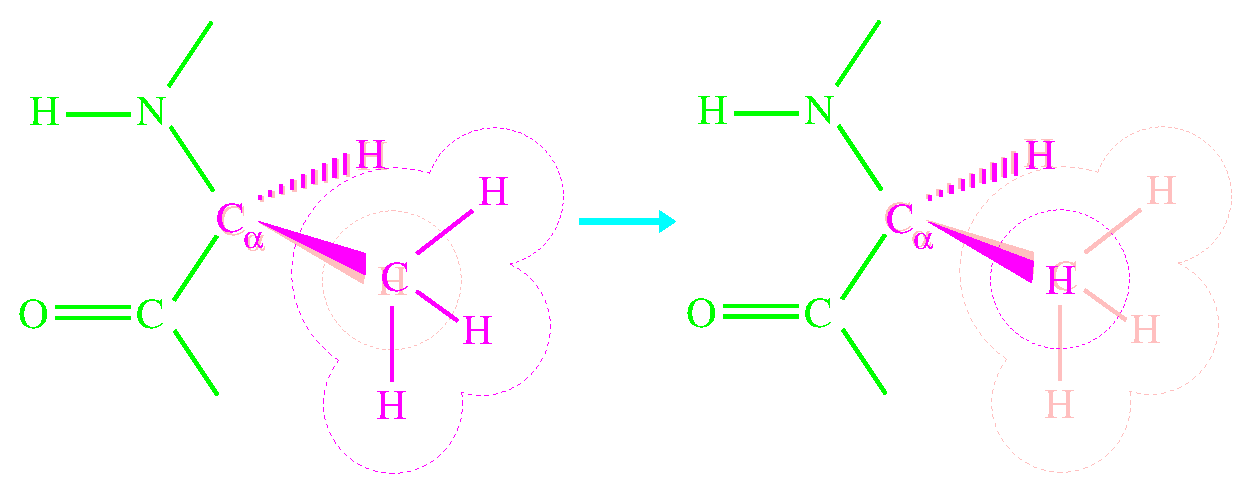
\includegraphics[width=14.5cm]{figures/dual_top}}
  \caption{Dual topology description for an alchemical simulation.
         Case example of the mutation of alanine into glycine.
         The lighter color denotes the non--interacting, alternate
         state.}
  \label{fig:dual_top}
\end{figure}


The charge and Lennard--Jones parameters of the alanine and
the glycine side chains
are defined as a function of $\lambda$, in such a fashion that 
the interaction of the methyl group of alanine with the rest of 
the protein is effective at the beginning of the simulation,
\ie $\lambda$ = 0, while
the glycine C$_\alpha$ hydrogen does not interact with the rest
of the protein, and {\it vice versa} at the end of the
simulation, \ie $\lambda$ = 1.
For intermediate values of $\lambda$, both the alanine and the glycine
side chains participate in non--bonded interactions with the rest 
of the protein, scaled on the basis of the current value of $\lambda$.
It should be emphasized that these side chains, however,
do not interact with themselves. Explicit care should be taken while
preparing the {\tt psf} file to exclude those atoms that are created
from those that will be annihilated in the course of the
\FEP\ calculation.


It is also worth noting that
the free energy calculation does not alter intramolecular
potentials, \ie bond stretch, valence angle deformation, torsions,
{\it etc}\dots, during
the simulation. In calculations targetted at the estimation
of free energy differences between two states characterized by
distinct environments --- \eg a ligand, bound to a protein in
the first simulation,
and solvated in water, in the second --- as is the 
case for most free energy calculations that make use of a thermodynamic 
cycle, perturbation of intramolecular terms can be safely
avoided.~\cite{Boresch.99a}


\subsubsection{Implementation of free energy perturbation in NAMD}


The procedure implemented in \NAMD\ is particularly
adapted for performing free 
energy calculations that split the $\lambda$
reaction path into a number of non--physical,
intermediate states, or ``windows''. Seperate simulations 
can be started for each window.
Alternatively, the {\sc Tcl} scripting ability of 
\NAMD\ can be employed advantageously
to perform the complete simulation in a single run.
An example making use of such script is supplied at the end 
of this user guide.


The following keywords can be used to control the alchemical free 
energy calculations. 

\begin{itemize}

\item
\NAMDCONFWDEF{fepOn}{ Is alchemical \FEP\ to be performed? }
{{\tt on} or {\tt off}}
{{\tt off}}
{Turns on parameter scaling and ensemble averaging for alchemical \FEP.}

\item
\NAMDCONF{lambda}{ Coupling parameter value }
{positive decimal between 0.0 and 1.0}
{The coupling parameter value determining the progress of the
perturbation. The non--bonded parameters of the atoms vanishing
in the course of the {\sc md} simulation are scaled by {\tt lambda}, whilst
the parameters of those atoms grown are scaled by (1-{\tt lambda}).}

\item
\NAMDCONF{dLambda}{Coupling parameter step}
{positive decimal between 0.0 and 1.0}
{The {\tt dLambda} value corresponds to the magnitude of the change in
the coupling parameter, $\lambda$, that defines the spacing between
adjacent windows.}

\item
\NAMDCONFWDEF{numFepEqlb}{Number of equilibration steps in the window, 
before data collection}
{positive integer less than {\tt numSteps} or {\tt run}}
{0}
{In each window {\tt numFepEqlb} steps of equilibration can be
performed before ensemble averaging is initiated. The output also contains
the data gathered during equilibration and is meant for analysis of
convergence properties of the \FEP\ calculation.}

\item
\NAMDCONFWDEF{fepFile}{{\sc pdb} file with perturbation flags}
{{\sc Unix} filename}
{coordinates}
{{\sc pdb} file to be used for indicating the \FEP\ status for each of
the atoms pertaining to the system. 
If this parameter is not declared specifically, then the
{\sc pdb} file containing the initial coordinates specified by
{\tt coordinates} is utilized for this information.}

\item
\NAMDCONFWDEF{fepCol}{Column in the {\tt fepFile} that carries 
                      the perturbation flag}
{X, Y, Z, O or B}
{O}
{Column of the {\sc pdb} file to use for retrieving the \FEP\ status 
of each atom, \ie a flag that indicates which atom will be perturbed
in the course of the simulation.
A value of {\tt -1} in the specified column indicates the atom will
vanish during the \FEP\ calculation, whereas a value of {\tt 1} 
indicates that the atom would grow.}

\item
\NAMDCONFWDEF{fepOutFreq}{Frequency of \FEP\ energy output in time--steps}
{positive integer}
{5}
{Every {\tt fepOutFreq} number of {\sc md} steps, the output file
{\tt fepOutFile} is updated by dumping energies that are
used for ensemble averaging.
This variable could be set to {\tt 1} to include all the 
configurations for ensemble averaging. Yet, it is recommended
to update {\tt fepOutFile}  energies with a
higher frequency 
to avoid large correlation between consecutive configurations.}

\item
\NAMDCONFWDEF{fepOutFile}{\FEP\ energy output filename}
{filename}
{outfilename}
{An output file named {\tt fepOutFile}.fep, generated by \NAMD,
contains the \FEP\ energies, dumped every {\tt fepOutFreq} steps.}

\item
\NAMDCONFWDEF{scaleH}{Perform Hamiltonian scaling }
{{\tt on} or {\tt off}}
{{\tt on}}
{Presently NAMD can perform Hamiltonian scaling based FEP simulation.
Amber (xleap) generated perturbation prmtop file is not supported
and parameter scaling based calculation cannot be performed with this
version.}

\end{itemize}


\subsubsection{Examples of input files for running FEP alchemical calculations}


The first example illustrates the use of {\sc Tcl} scripting for running
the alchemical \FEP\ feature of \NAMD: 

\begin{verbatim}
fepOn		on  
fepfile		ion.fep
fepCol		X
fepoutfile	ion.fepout
fepOutFreq	5
numFepEqlb	5000

set step 0.0
set dstep 0.1

while {$step <= 0.9} {
 firsttimestep	0
 lambda $step
 dlambda $dstep
 run  10000
 set step [expr $step+$dstep]
}
\end{verbatim}

Here, the {\sc pdb} file read by \NAMD\ to retrieve the information
about perturbed atoms is {\tt biotin.fep}. The pertinent information 
is present in the {\tt X} column. The output file of the free energy
calculation is {\tt biotinr.fepout}, in which energies are written
every {\tt 5} steps. No electrostatic decoupling is employed. 
$\delta \lambda$, the width of the windows, is set to {\tt 0.1}.
{\tt 5000} {\sc md} steps are performed in each window to
equilibrate the system. In this particular instance, 
the current value of $\lambda$
is controlled by the syntax {\tt set step}. 
The \FEP\ calculation is run until $\lambda$ reaches the
value {\tt 0.9}. In every window, {\tt 10000} {\sc md} steps
are being performed. At each value of $\lambda$, the first 
{\sc md} step is reset to {\tt 0} by means of the command
 {\tt firsttimestep}.


In the second example, each $\lambda$--state is declared
explicitly, avoiding the use of {\sc Tcl} scripting:

\begin{verbatim}
fepOn		on  
fepfile		ion.fep
fepCol		X
fepoutfile	ion.fepout
fepOutFreq	5
dLambda		0.1
numFepEqlb	5000

Lambda		0.0
run		10000

lambda		0.1
firsttimestep	0
run		10000
\end{verbatim}
$\vdots$
\begin{verbatim}
lambda		0.8
firsttimestep	0
run		10000

lambda		0.9
firsttimestep	0
run		10000
\end{verbatim}

The \FEP\ calculation is carried out from $\lambda$ = {\tt 0.0} to
{\tt 0.9}. In each new window, {\tt 10000} {\sc md} steps are
performed, and the number of steps is being reinitialized using
the {\tt firsttimestep} keyword.



\subsubsection{Description of \FEP\ simulation output }

The {\tt fepOutFile} contains electrostatic and van der Waals energy
data calculated for $\lambda$ and $\delta\lambda$, written every
{\tt fepOutFreq} steps. The column {\tt dE} is the energy
difference of the single configuration, {\tt dE\_avg} and {\tt dG}
are the instantaneous ensemble average of the energy and the calculated
free energy at the time step specified in column 2, respectively.
The temperature is specified in the penultimate column. On completion
of {\tt numFepEqlb} steps, the calculation of {\tt dE\_avg} and 
{\tt dG} is restarted. The accumulated net free energy change is output
and the end of the simulation at each lambda value. The cummulative
average energy {\tt dE\_avg} value may be summed using the 
trapezoidal rule to obtain an approximate TI estimate for the free 
energy change during the run.





\subsection{Locally Enhanced Sampling}
\label{section:les}

Locally enhanced sampling (LES)~\cite{ROIT91,SIMM98,SIMM00} increases
sampling and transition rates for a portion of a molecule by the use of
multiple non-interacting copies of the enhanced atoms.  These enhanced
atoms experience an interaction (electrostatics, van der Waals, and
covalent) potential that is divided by the number of copies present.
In this way the enhanced atoms can occupy the same space, while the
multiple instances and reduces barriers increase transition rates.

\subsubsection{Structure Generation}

To use LES, the structure and coordinate input files must be modified to
contain multiple copies of the enhanced atoms.  \PSFGEN\ provides the
{\tt multiply} command for this purpose.  \NAMD\ supports a maximum of 15
copies, which should be sufficient.  

Begin by generating the complete molecular structure and guessing
coordinates as described in Sec.~\ref{section:psfgen}.  As the last
operation in your script, prior to writing the psf and pdb files, add
the {\tt multiply} command, specifying the number of copies desired and
listing segments, residues, or atoms to be multiplied.  For example,
\verb#multiply 4 BPTI:56 BPTI:57# will create four copies of the last
two residues of segment BPTI.  You must include all atoms to be
enhanced in a single {\tt multiply} command in order for the bonded
terms in the psf file to be duplicated correctly.  Calling {\tt multiply}
on connected sets of atoms multiple times will produce unpredictable
results, as may running other commands after {\tt multiply}.

The enhanced atoms are duplicated exactly in the structure---they have
the same segment, residue, and atom names.  They are distinguished only
by the value of the B (beta) column in the pdb file, which is 0 for
normal atoms and varies from 1 to the number of copies created for
enhanced atoms.  The enhanced atoms may be easily observed in VMD with
the atom selection \verb#beta != 0#.

\subsubsection{Simulation}

In practice, LES is a simple method used to increase sampling;
no special output is generated.
The following parameters are used to enable LES:

\begin{itemize}

\item
\NAMDCONFWDEF{les}{is locally enhanced sampling active?}{{\tt on} or {\tt
off}}{{\tt off}}
{Specifies whether or not LES is active.}

\NAMDCONF{lesFactor}{number of LES images to use}
{positive integer equal to the number of images present}
{This should be equal to the factor used in {\tt multiply}
 when creating the structure.  The interaction potentials for images is
 divided by {\tt lesFactor}.  
}

\item
\NAMDCONFWDEF{lesReduceTemp}{reduce enhanced atom temperature?}{{\tt on} or {\tt
off}}{{\tt off}}
{Enhanced atoms experience interaction potentials divided by {\tt lesFactor}.
This allows them to enter regions that would not normally be thermally
accessible.  If this is not desired, then the temperature of these atoms
may be reduced to correspond with the reduced potential.  This option
affects velocity initialization, reinititialization, reassignment, and
the target temperature for langevin dynamics.  Langevin dynamics is
recommended with this option, since in a constant energy simulation energy
will flow into the enhanced degrees of freedom until they reach thermal
equilibrium with the rest of the system.  The reduced temperature atoms
will have reduced velocities as well, unless {\tt lesReduceMass} is also
enabled.}

\item
\NAMDCONFWDEF{lesReduceMass}{reduce enhanced atom mass?}{{\tt on} or {\tt off}}{{\tt off}}
{Used with {\tt lesReduceTemp} to restore velocity distribution to
enhanced atoms.  If used alone, enhanced atoms would move faster than
normal atoms, and hence a smaller timestep would be required.}

\item
\item
\NAMDCONFWDEF{lesFile}{PDB file containing LES flags}{UNIX filename} {{\tt coordinates}}
{PDB file to specify the LES image number of each atom.
If this parameter is not specified, then 
the PDB file containing initial coordinates specified by 
{\tt coordinates} is used.}

\item
\NAMDCONFWDEF{lesCol}{column of PDB file containing LES flags}{{\tt X}, {\tt Y}, {\tt Z}, {\tt O}, or {\tt B}}{{\tt B}}
{Column of the PDB file to specify the LES image number of each atom.
This parameter may specify any of the floating point fields of the PDB file, 
either X, Y, Z, occupancy, or beta-coupling (temperature-coupling).  
A value of 0 in this column indicates that the atom is not enhanced.
Any other value should be a positive integer less than {\tt lesFactor}.}

\end{itemize}


\subsection{Pair Interaction Calculations}
\label{section:pairinteraction}
\NAMD\ supportes the calculation of interaction energy calculations between 
two groups of atoms.  When enabled, pair interaction information will be
calculated and printed in the standard output file on its own line at the
same frequency as energy output.  The format of the line is
{\tt PAIR INTERACTION: STEP: {\it step} VDW\_FORCE: {\it fx fy fz} 
ELECT\_FORCE: {\it fx fy fz}}.
The displayed force is the force on atoms in group 1 and is units of 
kcal/mol/\AA. 

For trajectory analysis the 
recommended way to use this set of options is to use the NAMD Tcl scripting 
interface as described in Sec.~\ref{section:tclscripting} to run for
0 steps, so that NAMD prints the energy without performing any dynamics.

\begin{itemize}

\item
\NAMDCONFWDEF{pairInteraction}{is pair interaction calculation active?}
{{\tt on} or {\tt off}}{{\tt off}}
{Specifies whether pair interaction calculation is active.}

\item
\NAMDCONFWDEF{pairInteractionFile}{PDB file containing pair interaction flags}
{UNIX filename}{{\tt coordinates}}
{PDB file to specify atoms to use for pair interaction calculations.  If 
this parameter is not specified, then the PDB file containing initial 
coordinates specified by {\tt coordinates} is used.}

\item
\NAMDCONFWDEF{pairInteractionCol}{column of PDB file containing pair 
interaction flags}{{\tt X}, {\tt Y}, {\tt Z}, {\tt O}, or {\tt B}}{{\tt B}}
{
Column of the PDB file to specify which atoms to use for pair interaction
calculations.  This parameter may specify any of the floating point
fields of the PDB file, either X, Y, Z, occupancy, or beta-coupling
(temperature-coupling).  
}

\item
\NAMDCONFWDEF{pairInteractionSelf}{compute within-group interactions instead of
bewteen groups}{{\tt on} or {\tt off}}{{\tt off}}
{
When active, NAMD will compute bonded and nonbonded interactions only for atoms 
within group 1.  
}
 
\item
\NAMDCONF{pairInteractionGroup1}{Flag to indicate atoms in
group 1?}{integer}{}

\item
\NAMDCONF{pairInteractionGroup2}{Flag to indicate atoms in
group 2?}{integer}{}
{
These options are used to indicate which atoms belong to each interaction 
group.  Atoms with a value in the column specified by {\tt pairInteractionCol} 
equal to {\tt pairInteractionGroup1} will be assigned to group 1; likewise
for group 2.
}

\subsection{Pressure Profile Calculations}
\NAMD\ supports the calculation of lateral pressure profiles as a function of
the z-coordinate in the system.  The algorithm is essentially that described
by Lindahl and Edholm.  The simulation space is partitioned into slabs, and
the virial due to the interaction between two particles is distributed across 
the slabs containing the particles as well as the slabs that lie between the
particles (taking periodic boundary conditions into account).  The diagonal
components of the pressure tensor for each slab are recorded in the 
\NAMD\ output file.  The units of pressure are the same as in the regular 
\NAMD\ pressure output; i.e., bar.

The total virial contains contributions from three components: kinetic energy,
bonded interactions, and nonbonded interactions.  The kinetic and bonded 
components are easily calculated every timestep, and thus may be computed 
during a normal simulation run.  The nonbonded component, however, adds 
significant overhead and has not been implemented for PME calculations.  
The calculation of the nonbonded contribution should be performed offline,
using the saved frames of the trajectory file and a long nonbonded cutoff.

Pressure profile calculations may be performed in either constant volume 
or constant pressure conditions.  If constant pressure is enabled, the
slabs thickness will be rescaled along with the unit cell; the dcdUnitCell
option will also be switched on so that unit cell information is stored in
the trajectory file.

Periodic boundary conditions must also be enabled.


\item
\NAMDCONFWDEF{pressureProfile}{compute pressure profile}{{\tt on} or {\tt off}}{{\tt off}}
{
When active, NAMD will compute kinetic and bonded contributions to the 
pressure profile.  Results will be recorded in the \NAMD\ output file
in lines with the format
{\tt PRESSUREPROFILE: ts Axx Ayy Azz Bxx Byy Bzz ... }, where {\tt ts} is the
timestep, followed by the three diagonal components of the pressure tensor 
in the first
slab (the slab with lowest {\it z}), then the next lowest slab, and so forth.
NAMD will also output the pressure profile averaged over all the steps since
the last output.  The format of this line is 
{\tt PRESSUREPROFILEAVG: ts Axx Ayy Azz ... }; i.e., exactly as for the
instantaneous pressure.  It is recommended to use the averaged pressure profile
instead of the instantaneous value as this will give better statistics and
may prevent artifacts when using multiple timestepping.
}
\item
\NAMDCONFWDEF{pressureProfileSlabs}{Number of slabs in the spatial partition}{Positive integer}{10}{
\NAMD\ divides the entire periodic cell into horizontal slabs of equal 
thickness; {\tt pressureProfileSlabs} specifies the number of such slabs.
}

\item
\NAMDCONFWDEF{pressureProfileFreq}{How often to output pressure profile
data}{Positive integer}{1}{
Specifies the number of timesteps between output of pressure profile data.
}

\item
\NAMDCONFWDEF{pressureProfileNonbonded}{Compute nonbonded pressure profile
contribution}{{\tt on} or {\tt off}}{{\tt off}}{
When enabled, only the nonbonded contribution to the pressure profile will be
computed.  For trajectory analysis the 
recommended way to use this option is to use the \NAMD\ Tcl scripting 
interface as described in Sec.~\ref{section:tclscripting} to run for
0 steps, so that NAMD prints the pressure profile without performing any 
dynamics.
}
\end{itemize}

Here is an example snippet from a \NAMD\ input that can be used to compute
the nonbonded component of the pressure profile.  It assumes that the 
coordinates were saved in three dcd files ({\tt pp01.dcd}, {\tt pp02.dcd},
and {\tt pp03.dcd}) every 500 timesteps.  The {\tt pressureProfileSlabs}
must be the same as was used for the calculation of the bonded part of
the pressure.  Note the use of no switching function; this way the calculated
electrostatic energy will be closest to what would be calculated by PME.
\begin{verbatim}
switching	     off
cutoff		     20.0
pairlistdist   20.5

pressureProfile	on
pressureProfileSlabs 60 
pressureProfileFreq 100 
pressureProfileNonbonded on

# Assume that coordinates were written to the dcd files every 500 timesteps.
set ts 500
foreach dcd { pp01.dcd pp02.dcd pp03.dcd } {
  coorfile open dcd $dcd
  while { [coorfile read] != -1 } {
    firstTimestep $ts 
    run 0 
    incr ts 500
  }
  coorfile close
}
\end{verbatim}

